\scanpage{57}

\margin{\fbox{\parbox{.86\linewidth}{Seems to hold for any equivalence relation
\diagram{\begin{tikzcd}R\arrow[r,shift left]\arrow[r,shift right,"p"']&X\end{tikzcd}}
with ``geometric quotient'' $Y$, such that $p$ be \uline{smooth}, $X,Y$ be noeth---
Is \uuline{flat} enough??}}}
\mspage{-0.27-}

\uline{Proposition 0.9}: Let $S=\operatorname{Spec}(k)$, $k$ a field, and assume that
\figure{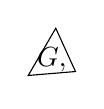
\begin{tikzpicture}[baseline=-.5ex]\node at (0,0) {$G$,};\draw (-.3,-.2)--(.3,-.15)--(.05,.4)--cycle;\end{tikzpicture}}
$X$ and $Y$ are algebraic schemes over $k$. If the action $\sigma$ is
\figure{
\begin{tikzpicture}[baseline=-.5ex]\node at (0,0) {free};\draw (0,0) ellipse (.4 and .25);\end{tikzpicture}},
and $(Y,\phi)$ is a geometric quotient of $X$ by $G$, then $X$ is a principal fibre bundle over $Y$ with group $G$.${}^*$

\margin{\figure{
\begin{tikzpicture}\draw (0,0) ellipse (.17 and .3);\end{tikzpicture}}\unsure{Dangerous} \unsure{example}?}
\margin{\figure{
\begin{tikzpicture}\draw (0,0)--(.2,.2)--(0,.4)--cycle;\end{tikzpicture}}$G$ \uline{smooth}$/k$!}

\uline{Proof}: First of all, we may assume that $k$ is algebraically closed: for by such a base extension, i) $\sigma$ remains free, ii) $(Y,\phi)$ remains a geometric quotient (Remark $\unsure{\gamma|7}$, \S2), iii) the property of being a principal fibre bundle descends (SGA 8, 5.4). Secondly, we may replace $Y$ by one of its local rings $\operatorname{Spec}(\underline{o}_{y,Y})$, for some closed point $y\in Y$: for all conditions of Definition 0.10 are expressible locally. And thirdly, we may replace $\operatorname{Spec}(\underline{o}_{y,Y})$ by $\operatorname{Spec}(\hat{\underline{o}}_{y,Y})$ (its completion). For this is also a faithfully flat quasi-compact base extension and, as before, i) $\sigma$ remains free, ii) $(Y,\phi)$ remains a geometric quotient, and iii) the property of being a principal fibre bundle descends.

Therefore we have $Y=\operatorname{Spec}(A)$, where $A$ is a complete local ring with algebraically closed residue field. Let $y$ be the closed point of $Y$, and let $x$ be a closed, hence $k$-rational point of $X$ over $y$. Let $I_x\subset\underline{o}_{x,X}$ be
\figure{
\begin{tikzpicture}[baseline=-.5ex]\node at (0,0) {the};\draw (0,0) ellipse (.28 and .35);\end{tikzpicture}}
ideal defining
\figure{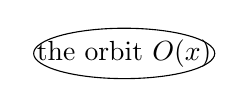
\begin{tikzpicture}[baseline=-.5ex]\node at (0,0) {the orbit $O(x)$};\draw (0,0) ellipse (1.15 and .32);\end{tikzpicture}}
of $x$. Since $\sigma$ is free, the morphism $\psi_x$ defines an isomorphism:
\[
\underline{o}_{x,X}/I_x\xrightarrow{\sim}\underline{o}_{e,G}.
\]
\margin{ambiguous}

\noindent\rule{2cm}{.4pt}

${}^*$It seems very likely that this result holds even if we do not assume \uline{a priori} that $Y$ is an algebraic scheme; and that it then follows \uline{a posteriori} that $Y$ is an algebraic scheme.

\margin{56}
